\documentclass[12pt, letterpaper, preprint, comicneue]{aastex63}
%\usepackage[default]{comicneue} % comic sans font for editing
\usepackage[T1]{fontenc}
%%% This file is generated by the Makefile.
\newcommand{\giturl}{\url{https://github.com/changhoonhahn/provabgs}}
\newcommand{\githash}{6d00025}\newcommand{\gitdate}{2021-01-14}\newcommand{\gitauthor}{ChangHoon Hahn}

\usepackage{color}
\usepackage{amsmath}
\usepackage{natbib}
\usepackage{ctable}
\usepackage{bm}
\usepackage[normalem]{ulem} % Added by MS for \sout -> not required for final version
\usepackage{xspace}
\usepackage{csvsimple} 

\usepackage{graphicx}
\usepackage{pgfkeys, pgfsys, pgfcalendar}


% typesetting shih
\linespread{1.08} % close to 10/13 spacing
\setlength{\parindent}{1.08\baselineskip} % Bringhurst
\setlength{\parskip}{0ex}
\let\oldbibliography\thebibliography % killin' me.
\renewcommand{\thebibliography}[1]{%
  \oldbibliography{#1}%
  \setlength{\itemsep}{0pt}%
  \setlength{\parsep}{0pt}%
  \setlength{\parskip}{0pt}%
  \setlength{\bibsep}{0ex}
  \raggedright
}
\setlength{\footnotesep}{0ex} % seriously?

% citation alias

% math shih
\newcommand{\setof}[1]{\left\{{#1}\right\}}
\newcommand{\given}{\,|\,}
\newcommand{\lss}{{\small{LSS}}\xspace}

\newcommand{\Om}{\Omega_{\rm m}} 
\newcommand{\Ob}{\Omega_{\rm b}} 
\newcommand{\OL}{\Omega_\Lambda}
\newcommand{\smnu}{M_\nu}
\newcommand{\sig}{\sigma_8} 
\newcommand{\mmin}{M_{\rm min}}
\newcommand{\BOk}{\widehat{B}_0} 
\newcommand{\hmpc}{\,h/\mathrm{Mpc}}
\newcommand{\bfi}[1]{\textbf{\textit{#1}}}
\newcommand{\parti}[1]{\frac{\partial #1}{\partial \theta_i}}
\newcommand{\partj}[1]{\frac{\partial #1}{\partial \theta_j}}
\newcommand{\mpc}{{\rm Mpc}}
\newcommand{\eg}{\emph{e.g.}}
\newcommand{\ie}{\emph{i.e.}}

% cmds for this paper 
\newcommand{\gr}{g{-}r}
\newcommand{\fnuv}{FUV{-}NUV}
\newcommand{\sfr}{{\rm SFR}}
\newcommand{\ssfr}{{\rm SSFR}}
\newcommand{\mtaum}{m_{\tau,M_*}}
\newcommand{\mtaus}{m_{\tau,{\rm SSFR}}}
\newcommand{\ctau}{c_\tau}
\newcommand{\mdeltam}{m_{\delta,M_*}}
\newcommand{\mdeltas}{m_{\delta,{\rm SFR}}}
\newcommand{\cdelta}{c_\delta}
\newcommand{\eda}{EDA}


\newcommand{\specialcell}[2][c]{%
  \begin{tabular}[#1]{@{}c@{}}#2\end{tabular}}
% text shih
\newcommand{\foreign}[1]{\textsl{#1}}
\newcommand{\etal}{\foreign{et~al.}}
\newcommand{\opcit}{\foreign{Op.~cit.}}
\newcommand{\documentname}{\textsl{Article}}
\newcommand{\equationname}{equation}
\newcommand{\bitem}{\begin{itemize}}
\newcommand{\eitem}{\end{itemize}}
\newcommand{\beq}{\begin{equation}}
\newcommand{\eeq}{\end{equation}}

%% collaborating
\newcommand{\todo}[1]{\marginpar{\color{red}TODO}{\color{red}#1}}
\definecolor{orange}{rgb}{1,0.5,0}
\newcommand{\ch}[1]{{\color{orange}{\bf CH:} #1}}

\begin{document} \sloppy\sloppypar\frenchspacing 

\title{PROVABGS Probabilistic Stellar Mass Function of the BGS One-Percent
Survey} 
\date{\texttt{DRAFT~---~\githash~---~\gitdate~---~NOT READY FOR DISTRIBUTION}}

\newcounter{affilcounter}
\author{ChangHoon Hahn}
\altaffiliation{changhoon.hahn@princeton.edu}
\affil{Department of Astrophysical Sciences, Princeton University, Peyton Hall, Princeton NJ 08544, USA} 

\begin{abstract}
    We present the probabilistic stellar mass function (pSMF) of galaxies in
    the DESI Bright Galaxy Survey (BGS), observed as part of the One-Percent Survey. 
    We derive the pSMF from posteriors of stellar mass, $M_*$, for all the BGS
    galaxies using statistically rigorous hierarchical inference.
    The $M_*$ posteriors are inferred from DESI photometry and spectroscopy
    using the \cite{hahn2022} PROVABGS SED modeling framework. 
    We 
\end{abstract}

\keywords{
keyword1 -- keyword2 -- keyword3
}

% --- intro ---  
\section{Introduction} \label{sec:intro} 

% --- observations ---  
\section{The DESI Bright Galaxy Survey: One-Percent Survey}  \label{sec:edr}
DESI began its five years of operations in May 14, 2021. 
%\todo{something about EDR}
Before its start, DESI conducted the Survey Validation (SV) campagin to verify
that the survey will meets its scientific and performance
requirements. 
The SV campaign was divided into two main programs: the first, SV1,
characterized the survey's performance for different observing conditions and
was used to optimize sample selection. 
The second, the One-Percent Survey (or SV3), observed a dataset that can be
used for representative clustering measurements and deliver a ‘truth’ sample
with high completeness over an area at least 1\% of the expected main survey
footprint.
We refer readers to \cite{sv_paper} for details on the DESI SV programs.
In this work, we focus on BGS galaxies observed during the One-Percent Survey.

The One-Percent Survey observed on 38 nights from April 2021 to the end of 
May 2021.
During this time DESI observed 288 bright time exposures that cover 214 BGS
`tiles', planned DESI pointings. 
The tiles were arranged so that a set of 11 overlapping tiles has their centers 
arranged around a 0.12 deg circle, forming a ‘rosette’ completeness pattern. 
In total, the One-Percent Survey observed 20 rosettes covering 180 
${\rm deg}^2$ spanning the northern galactic cap (see Figure 1 in
\citealt{hahn2022}).  

All BGS spectra observed during the One-Percent Survey are reduced using the
`Fuji' version of the DESI spectroscopic data reduction
pipeline~\citep{guy2022}. 
First, spectra are extracted from the spectrograph CCDs using the 
{\em Spectro-Perfectionsim} algorithm of \cite{bolton2010}.
Then, fiber-to-fiber variations are corrected by flat-fielding and a sky model,
empirically derived from sky fibers, is subtracted from each spectrum.
Afterwards, the fluxes in the spectra are calibrated using stellar model fits
to standard stars. 
The final processed spectra is then derived by co-adding the calibrated spectra
across expoures of the same tile. 
In total, DESI observed spectra of 155,022 BGS Bright and 109,418 BGS Faint 
targets during the One-Percent Survey. 

For each spectrum, redshift is measured using 
{\sc Redrock}\footnote{https://redrock.readthedocs.io}~\citep{bailey2022}, 
a redshift fitting algorithm that uses $\chi^2$ minimization computed from a
linear combination of Principal Component Analysis (PCA) basis spectral
templates in three template classes (``stellar'',  ``galaxy'', and ``quasar'').
{\sc Redrock} also provides measures of redshift uncertainty, $\mathtt{ZERR}$
and redshift confidence, $\Delta\chi^2$, which corresponds to the difference
between the $\chi^2$ values of the best-fit model and the next best-fit model.
We restrict our sample to galaxy targets with reliable redshift measurements.
We only keep targets with spectra classified as galaxy spectra by 
{\sc Redrock}, no {\sc Redrock} warning flags, $\Delta\chi^2 > 40$,
and {\sc Redrock} redshift uncertainty $\mathtt{ZERR} < 0.0005 (1 + z)$.
We also exclude any targets observed using malfunctioning fiber positioners.
Lastly, we impose a redshift range of $0 < z < 0.6$.  
After these cuts, our One-Percent Survey BGS sample includes 143,074 BGS Bright
galaxies and 96,771 BGS Faint galaxies.

% --- methods ---  
\section{PROVABGS SED Modeling} \label{sec:provabgs}
% brief explanation of the PROVABGS SED modeling 
For each BGS EDR galaxy, we derive its $M_*$ and other properties,
$\overline{\rm SFR}$, $Z_{\rm MW}$, and $t_{\rm age, MW}$ from DESI
photometry and spectroscopy using the PROVABGS SED modeling
framework~\citep{hahn2022}.  
PROVABGS models galaxy SEDs using stellar population synthesis with
non-parametric star-formation history (SFH) with a starburst, a non-parametric
metallicity history (ZH) that varies with time, and a flexible dust
attenuation prescription.
The non-parameteric SFH and ZH prescriptions are derived from SFHs and ZHs of
simulated galaxies in the Illustris hydrodynamic
simulation~\citep{vogelsberger2014, genel2014, nelson2015} and provide compact 
and flexibly representations of SFHs and ZHs.
For the stellar population synthesis, PROVABGS uses the Flexible Stellar
Population Synthesis~\citep[FSPS;][]{conroy2009, conroy2010b} model with MIST
isochrones~\citep{paxton2011, paxton2013, paxton2015, choi2016, dotter2016},
\cite{chabrier2003} initial mass function (IMF), and a combination of
MILES~\citep{sanchez-blazquez2006} and BaSeL~\citep{lejeune1997, lejeune1998,
westera2002} spectral libraries.

Furthermore, PROVABGS provides a Bayesian inference framework for inferring
full posterior probability distributions of the SED model parameter:
$p(\theta\given {\bf X}^{\rm photo}, {\bf X}^{\rm spec})$, where ${\bf X}^{\rm
photo}$ represents the photometry and ${\bf X}^{\rm spec}$ represents the
spectroscopy. 
In total, $\theta$ has 13 parameters: $M_*$, 6 parameters specifying the SFH
($\beta_1, \beta_2, \beta_3, \beta_4, f_{\rm burst}, t_{\rm burst}$), 2
parameters specifying ZH ($\gamma_1, \gamma_2$), 3 parameters specifying
dust attenuation ($\tau_{\rm BC}, \tau_{\rm ISM}, n_{\rm dust}$), and a
nuisance parameter for the fiber aperture effect. 
Posteriors have distinct advantages over point estimates because they
accurately estimate uncertainties and degeneracies among galaxy properties.
Furthermore, as we later demonstrate, they are essential for principled
population inference: \eg~SMF.  

In practice, accurately estimating a 13 dimensional posterior requires a large
number ($\gtrsim$100,000) SED model evaluations, which would require
prohibitive computational resources. 
To address this challenge, PROVABGS samples the posterior using the
\cite{karamanis2020} ensemble slice Markov Chain Monte Carlo (MCMC) sampling
with the {\sc zeus} Python package\footnote{https://zeus-mcmc.readthedocs.io/}.
PROVABGS further accelerates the inference by using neural emulators for the
SED models. 
The emulators are accurate to subpercent level and $>100\times$ faster than the
original SED model based on FSPS~\citep{kwon2022}. 
With {\sc zeus} and neural emulation, deriving a posterior takes $\sim$5 min
per galaxy with PROVABGS.
Moreover, \cite{hahn2022} demonstrated PROVABGS can accurately infer $M_*$
overall the full expected $M_*$ range of BGS, using forward modeled synthetic
DESI observations. 

\begin{figure}
\begin{center}
    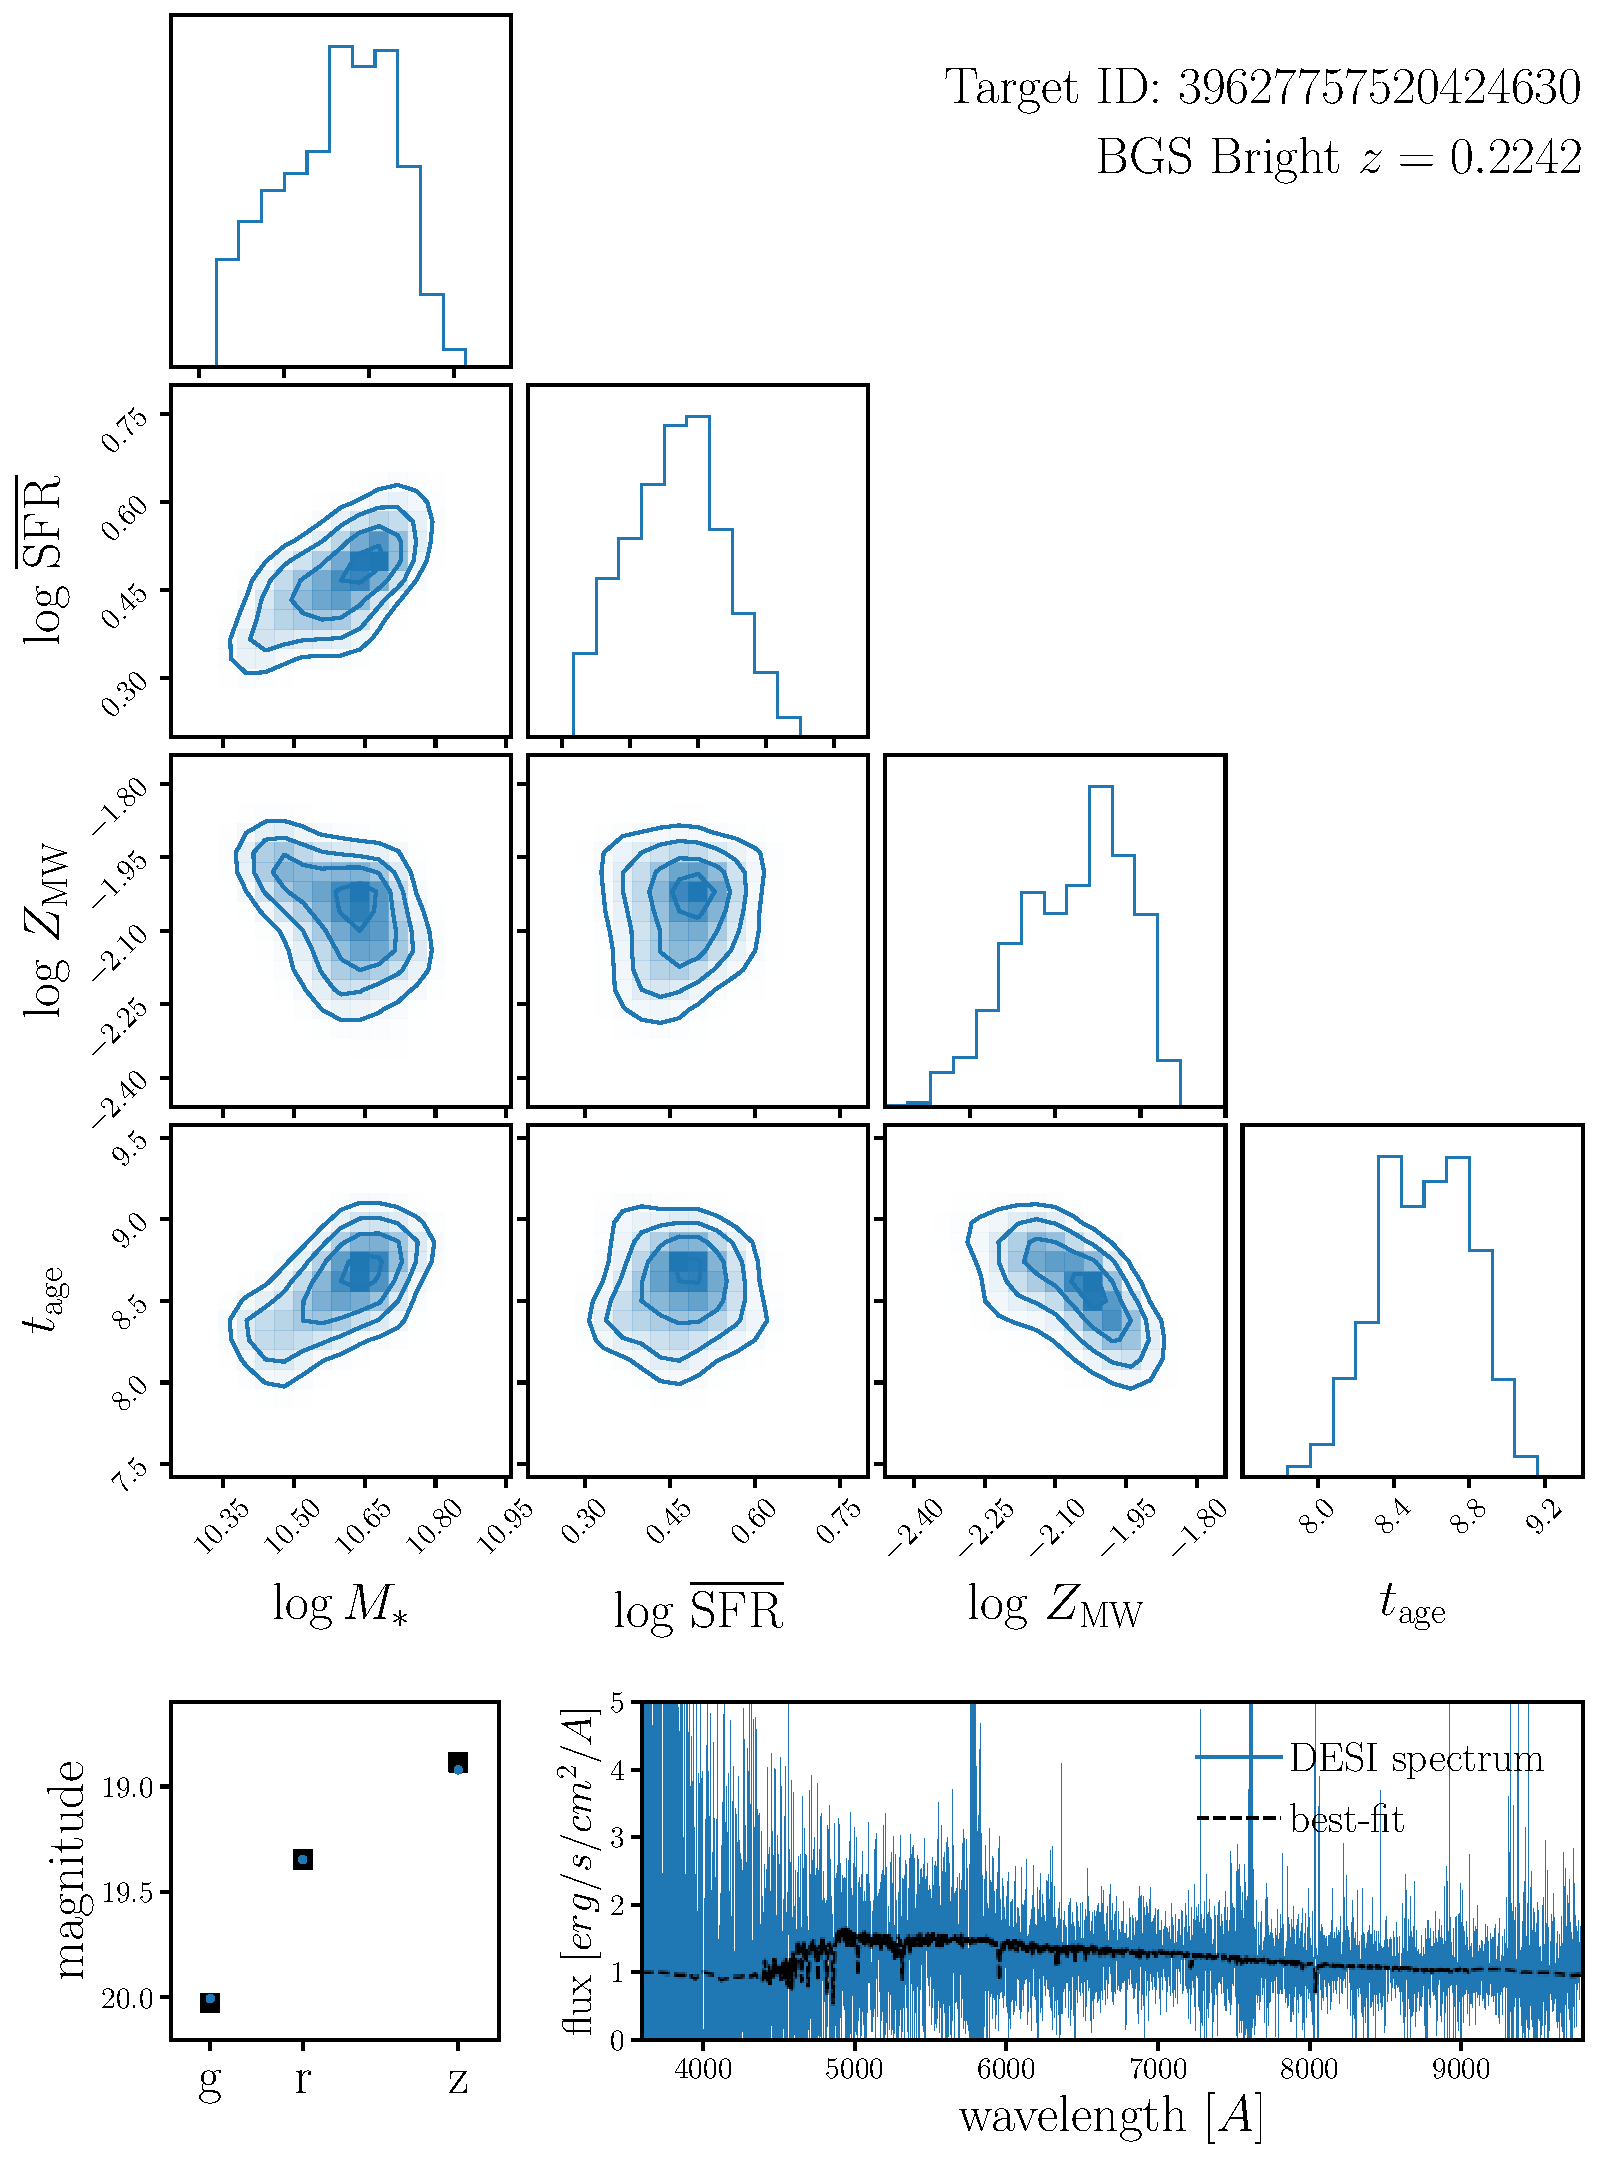
\includegraphics[width=0.6\textwidth]{figs/provabgs_posterior.pdf}
    \caption{
    }\label{fig:posterior}
\end{center}
\end{figure}


\begin{figure}
\begin{center}
    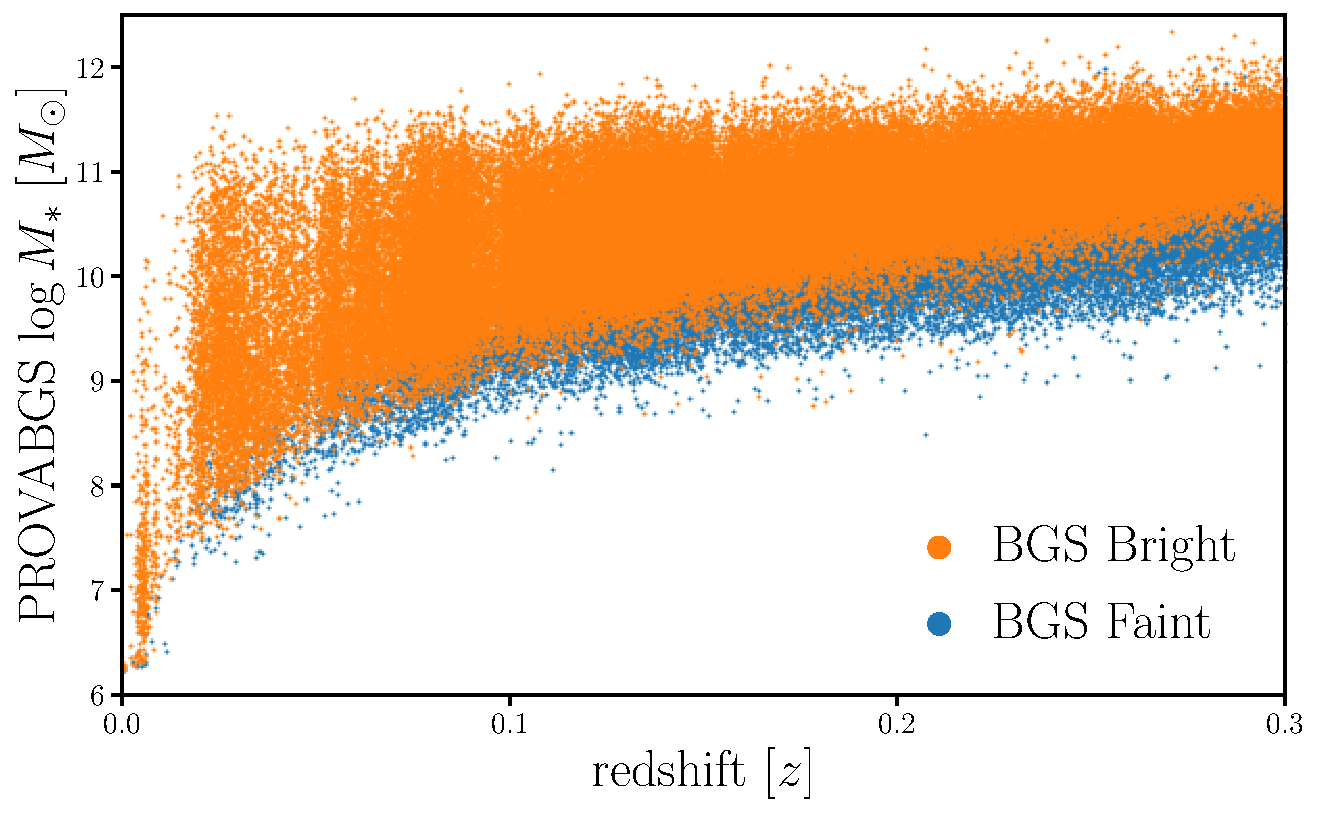
\includegraphics[width=0.6\textwidth]{figs/mstar_z.pdf}
    \caption{
    }\label{fig:mstar_z}
\end{center}
\end{figure}


In Figure~\ref{fig:posterior}, 

Figure~\ref{fig:mstar_z},

% --- results ---  
\section{Results} \label{sec:results}
We are interested in estimating the SMF of BGS galaxies from their individual
marginalized posteriors, $p(M_* \given {\bfi X_i})$, derived using
PROVABGS~(Section~\ref{sec:provabgs}). 

we're going to do population inference in a hierarchical bayesian framework and
use a normalizing flow.
%We can infer the population hyperparameters, μ∆θ and σ∆θ , using a hierarchical Bayesian framework (e.g. Hogg et al. 2010; Foreman-Mackey et al. 2014; Baronchelli et al. 2020).

why? because it produces unbiased inference. 

why do we use normalizing flows? 

We follow the same approach as \cite{hahn2022} to estimate:
\begin{align}\label{eq:popinf}
p(\phi \given \{{\bfi X_i}\}) 
    =&~\frac{p(\phi)~p( \{{\bfi X_i}\} \given \phi)}{p(\{{\bfi X_i}\})}\\
    =&~\frac{p(\phi)}{p(\{{\bfi X_i}\})}\int p(\{{\bfi X_i}\} \given \{\theta_i\})~p(\{\theta_i\} \given \phi)~{\rm d}\{\theta_i\}.\\
    =&~\frac{p(\phi)}{p(\{{\bfi X_i}\})}\prod\limits_{i=1}^N\int p({\bfi X_i} \given \theta_i)~p(\theta_i \given \phi)~{\rm d}\theta_i\\
    =&~\frac{p(\phi)}{p(\{{\bfi X_i}\})}\prod\limits_{i=1}^N\int \frac{p(\theta_i \given {\bfi X_i})~p({\bfi X_i})}{p(\theta_i)}~p(\theta_i \given \phi)~{\rm d}\theta_i\\
    =&~p(\phi)\prod\limits_{i=1}^N\int \frac{p(\theta_i \given {\bfi X_i})~p(\theta_i \given \phi)}{p(\theta_i)}~{\rm d}\theta_i. 
\intertext{
    We estimate the integral using $S_i$ Monte Carlo samples from the
    individual posteriors $p(\theta_i \given {\bfi X_i})$: 
}
    \approx&~p(\phi)\prod\limits_{i=1}^N\frac{1}{S_i}\sum\limits_{j=1}^{S_i}
    \frac{p(\theta_{i,j} \given \phi)}{p(\theta_{i,j})}.
\end{align} 

BGS provides two samples: BGS Bright and Faint. 
Galaxies in BGS Bright are selected based on a $r < 19.5$ flux limit, while
the ones in BGS Faint are selected based on a fiber-magnitude and color limit
and $r < 20.0175$ flux limit. 
Since neither of these samples are volume-limited and complete as a function
of $M_*$, we must include the selection effect when estimating the SMF. 
We do this by including weights derived from $z^{\rm max}$, the maximum
redshift that galaxy $i$ could be placed and still be included in the BGS
samples. 
We derive $z^{\rm max}_i$ for every galaxy using by redshifting the SED
predicted by the best-fit parameters. 
We then derive $V^{\rm max}_i$, the comoving volume out to $z^{\rm max}_i$, and
weights $w_i = w_{i, {\rm comp}}/V^{\rm max}_i$. 
We modify Eq.~\ref{eq:popinf} to include $w_i$: 
\begin{align}
p(\phi \given \{{\bfi X_i}\}) 
    \approx&~\frac{p(\phi)}{\prod\limits_{i=1}^N p({\bfi X_i})^{w_i}} 
    \prod\limits_{i=1}^N \left(\int p({\bfi X_i} \given \theta_i)~p(\theta_i \given \phi)~{\rm d}\theta_i \right)^{w_i} \\ 
    \approx&~\frac{p(\phi)}{\prod\limits_{i=1}^N p({\bfi X_i})^{w_i}} 
    \prod\limits_{i=1}^N \left( \sum\limits_{j=1}^{S_i}
    \frac{p(\theta_{i,j} \given \phi)}{p(\theta_{i,j})} \right)^{w_i} \\
    \approx&~\frac{p(\phi)}{\prod\limits_{i=1}^N p({\bfi X_i})^{w_i}} 
    \prod\limits_{i=1}^N \left( \sum\limits_{j=1}^{S_i}
    \frac{q_\phi(\theta_{i,j})}{p(\theta_{i,j})} \right)^{w_i}.
\end{align} 

In practice, we do not derive the full posterior 
$p(\phi \given \{{\bfi X_i}\})$. 
Instead we derive the maximum a posteriori (MAP) hyperparameter 
$\phi_{\rm MAP}$ that maximizes $p(\phi \given \{{\bfi X_i}\})$ or 
$\log p(\phi \given \{{\bfi X_i}\})$.
We expand, 
\begin{align}
\log p(\phi \given \{{\bfi X_i}\}) 
    \approx&~\log p(\phi) + % \sum\limits_{i=1}^N w_i \log w_i + 
    \sum\limits_{i=1}^N w_i \log \left(\sum\limits_{j=1}^{S_i} \frac{q_\phi(\theta_{i,j})}{p(\theta_{i,j})} \right).
\end{align} 
Since the first two terms are constant, we derive $\phi_{\rm MAP}$ by
maximizing 
\begin{equation}
    \max_\phi~~\sum\limits_{i=1}^N w_i \log \left(\sum\limits_{j=1}^{S_i} \frac{q_\phi(\theta_{i,j})}{p(\theta_{i,j})} \right).
\end{equation}
We use {\sc Adam} optimizer and determine the architecture of the normalizing
flow through experimentation.  

paragraph summarizing the weights that we use: vmax, spectroscopic completeness
weights, 


%\approx&~\log p(\phi) - 
%\log \prod\limits_{i=1}^N p({\bfi X_i})^{w_i} + 
%\log \prod\limits_{i=1}^N \left(\int p({\bfi X_i} \given \theta_i)~p(\theta_i \given \phi)~{\rm d}\theta_i \right)^{w_i} \\
%\approx&~\log p(\phi) - 
%\sum\limits_{i=1}^N w_i \log p({\bfi X_i}) + 
%\sum\limits_{i=1}^N w_i \log \left(\int p({\bfi X_i} \given \theta_i)~p(\theta_i \given \phi)~{\rm d}\theta_i \right) \\
%\approx&~\log p(\phi) + 
%\sum\limits_{i=1}^N w_i \log \left(\frac{1}{w_i} \sum\limits_{j=1}^{S_i} w_{i,j} \frac{p(\theta_{i,j} \given \phi)}{p(\theta_{i,j}} \right) \\


%\subsection{Targeting Completeness} \label{sec:ts}
% https://desi.lbl.gov/trac/wiki/ClusteringWG/LSScat/SV3/version2.1/fulldat
% https://desi.lbl.gov/trac/wiki/ClusteringWG/LSScat/SV3/version2.1/fullran


\subsection{The Probabilistic Stellar Mass Function} \label{sec:psmf}


% --- summary ---  
\section{Summary and Discussion} \label{sec:summary}



discussion of BGS in the DESI main survey


\todo{mention federico's paper as subsequent work with schetcher function fits} 

In subsequent work we will extend the hierarhical inference framework in 
this work to the SFR-$M_*$ distribution and present the probabilistic 
SFR-$M_*$ distribution and quiescent fraction. 



\section*{Acknowledgements}
It's a pleasure to thank

\appendix
\section{Spectroscopic Completeness} \label{sec:spec_comp}
Spectroscopic galaxy surveys, such as BGS, do not successfully measure the
redshift for all of the galaxies they target. 
As a result, this spectroscopic incompleteness must be accounted for when
measuring galaxy population statistics such as the SMF.  
In this appendix, we present how we estimate the spectroscopic incompleteness
for BGS and derive the weights we use to correct for its impact on the SMF. 

For BGS, spectroscopic incompleteness is primarily driven by fiber assignment
and redshift failures.  
DESI uses 10 fiber-fed spectrographs with 5000 fibers but targets more galaxies
than available fibers. 
For instance, the BGS Bright and Faint samples have $\sim 860$ and 
$530\,{\rm targets}/{\rm deg}^2$, respectively. 
For the 8 ${\rm deg}^2$ field-of-view of DESI, this roughly correspond to
11,000 targets, significantly more than the 5000 available fibers. 
DESI only measures the spectra of targets that are assigned fibers. 
In fact, of the 5000, a minimum of 400 ‘sky’ fibers are dedicated to measuring
the sky background for accurate sky subtraction and an additional 100 fibers
are assigned to standard stars for flux calibration~\cite{guy2022}.

Furthermore, each fiber is controlled by a robotic fiber positioner on the
focal plane. 
These positioners can rotate on two arms and be positioned within a circular
patrol region of radius 1.48 arcmin~\citep{schubnell2016, desi2016a,2022b, silber2022}.
Although the patrol regions of adjacent positioners slightly overlap, the
geometry of the positioners cause higher incompleteness in regions with high
target density~\citep{smith2019}.
To mitigate the incompleteness from the fiber assignment, BGS will observe its  
footprint with four passes.
With this strategy, BGS achieves $\sim$80\% fiber assignment
completeness~\citep{hahn_bgs}.

To estimate fiber assignment completeness, we run the fiber assignment
algorithm~\citep{raichoor2022} on BGS targets 128 separate times.
For each BGS galaxy, $i$, we count the total number of times out of 128 that
the galaxy is assigned a fiber: $N_{i, {\rm FA}}$. 
Then to correct for the fiber assignment incompleteness, we assign correction
weights
\begin{equation} \label{eq:w_fa}
    w_{i, \mathrm{FA}} = \frac{128}{N_{i, \mathrm{FA}}}
\end{equation}
to each BGS galaxy. 

\begin{figure}[h]
\begin{center}
    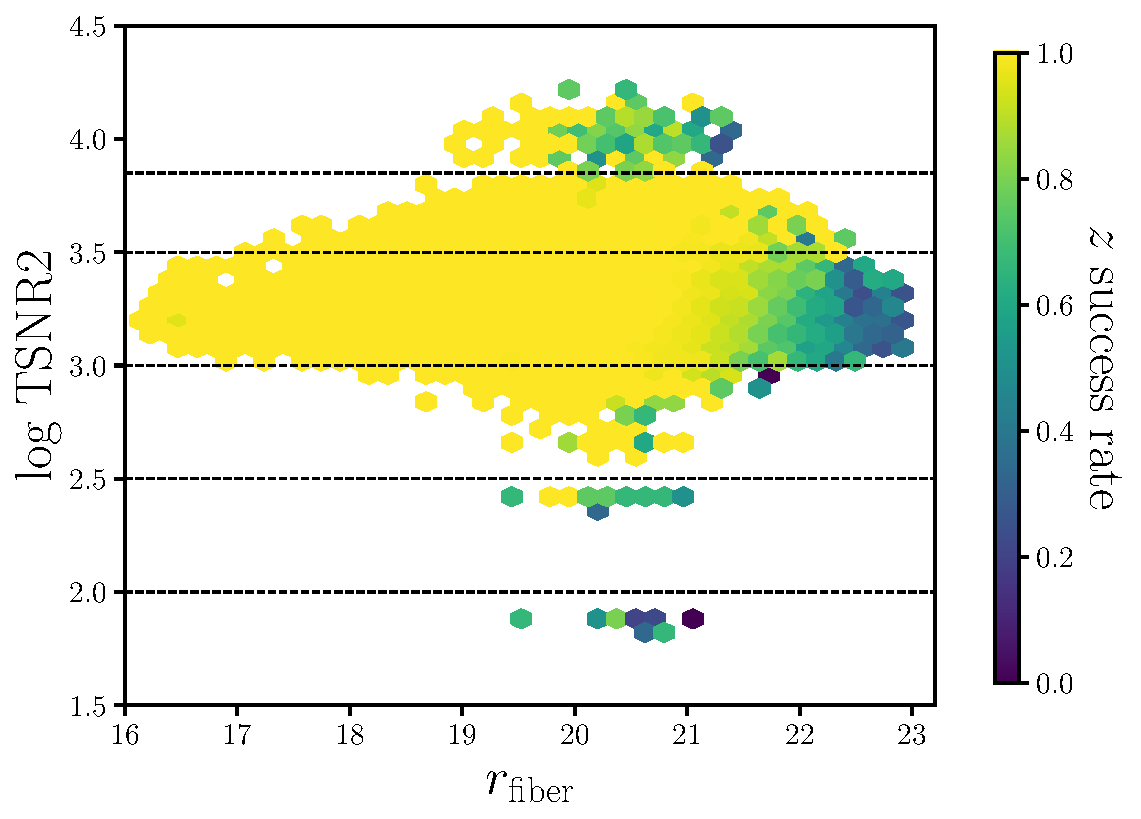
\includegraphics[width=0.5\textwidth]{figs/bgs_bright_rfib_tsnr2.pdf} 
    \caption{
        Redsift success rate of BGS Bright galaxies as a function of 
        $r_{\rm fiber}$ and TSNR2.
        TSNR2 is a statistic that roughly corresponds to the signal-to-noise
        ratio of the observed spectrum. 
        The color map represents the mean redshift success rate in each hexbin.
        We mark the TSNR2 bins (black dashed) that we use to separately fit the
        redshift success rate as a function of $r_{\rm fiber}$ using
        Eq.~\ref{eq:zsucc}.
        In each TSNR2 bin, redshift success decreases as $r_{\rm fiber}$
        increases. 
    }\label{fig:zfail0}
\end{center}
\end{figure}

Although we measure a spectrum for each galaxy assigned a fiber, we do not
accurately measure a redshift for every spectra. 
This redshift measurement failure significantly contributes to spectroscopic
incompleteness. 
For BGS, redshift failure of an observed galaxy spectrum depends mainly on
fiber magnitude and a statistic, TSNR2.
Fiber magnitude is derived from the predicted flux of the BGS object within a
1.5\arcsec diameter fiber; we use $r$-band fiber magnitude $r_{\rm fiber}$. 
TSNR2 roughly corresponds to the signal-to-noise ratio of the spectrum and is 
used to calibrate the effective exposure times in DESI observations

In Figure~\ref{fig:zfail0}, we present the redshift success rate of BGS Bright
galaxies as a function of $r_{\rm fiber}$ and TSNR2.

\begin{equation} \label{eq:zsucc}
    f_{z-{\rm success}}(r_{\rm fiber}) = \frac{1}{2} \left(1-{\rm erf}(c_0 (r_{\rm fiber} - c_1))\right)
\end{equation}


\begin{figure}
\begin{center}
    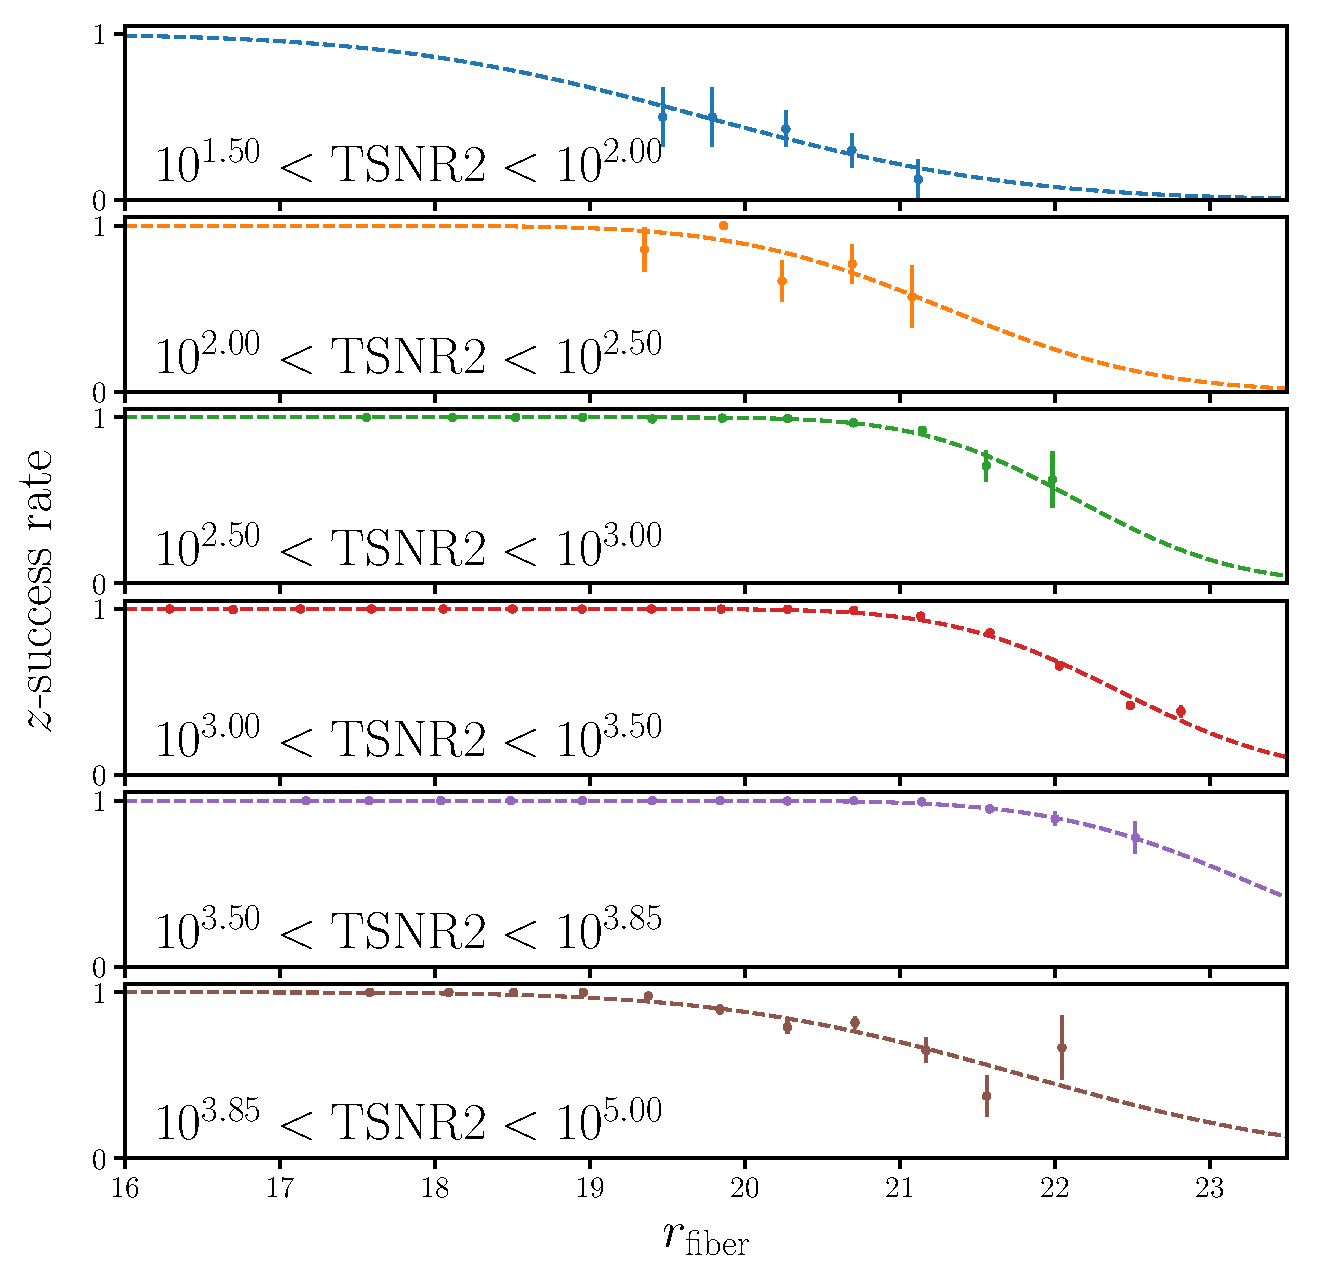
\includegraphics[width=0.5\textwidth]{figs/bgs_bright_rfib_tsnr2_zsuccess.pdf}
    \caption{
        Redshift success rates of BGS Bright galaxies  as a function of 
        $r_{\rm fiber}$ in 6 TSNR2 bins. 
        The error bars represent the poisson uncertainties.
        In each panel, we include the best-fit analytic (Eq.~\ref{eq:zsucc})
        approximation of the redshift success rate (dashed). 
        The best-fit $c_0$ and $c_1$ values are derived using $\chi^2$
        minimization. 
        We use this analytic approximation to calculate the spectroscopic
        completeness weights.
    }\label{fig:zfail1}
\end{center}
\end{figure}
% --- references ---
% https://desi.lbl.gov/trac/wiki/ClusteringWG/LSScat/DA02main/current_version#clusteringfiles


\begin{figure}
\begin{center}
    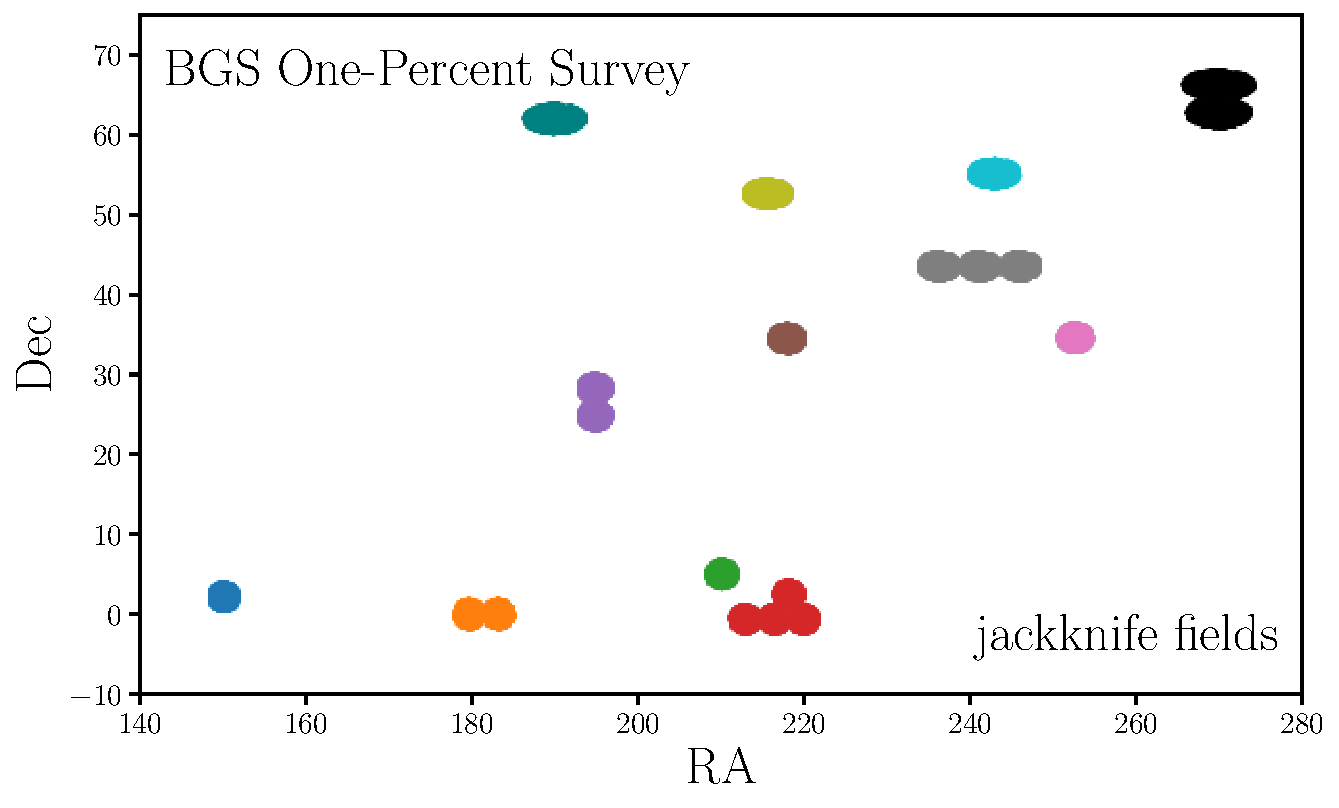
\includegraphics[width=0.5\textwidth]{figs/jackknife_fields.pdf} 
    \caption{
        The RA and Dec of the 12 jackknife fields of the BGS One-Percent Survey
        used to estimate the uncertainties on the SMF from sample variance. 
        We mark each field with a distinct color. 
    }\label{fig:jack}
\end{center}
\end{figure}


\section{Uncertainties on the SMF} \label{sec:jack}
We estimate the uncertainties of the SMF from sample variance using the
standard jackknife technique. 
This involves splitting our BGS sample into subsamples and then estimating
uncertainties using the subsample-to-subsample variations:  
\begin{equation} \label{eq:jack} 
    \sigma_\Phi = \left(\frac{N_{\rm jack}-1}{N_{\rm jack}}
    \sum\limits_{k=1}^{N_{\rm jack}} (\Phi_k - \Phi)^2 \right).
\end{equation} 
$N_{\rm jack}$ is the number of jackknife subsamples and $\Phi_k$ represents
the SMF estimated from the BGS galaxies excluding the jackknife subample $k$. 
In this work, we split the BGS sample into 12 jackknife fields based on the
angular positions of galaxies. 
We present the jackknife fields in Figure~\ref{fig:jack} with distinct colors. 

\section{Stellar Mass Completeness} \label{sec:mscomp}

First, we take galaxies with $i \Delta z < z < (i+1) \Delta z$. 

For each galaxy take their best-fit SED from {\sc PROVABGS} and artificially redshift it to 
$z' = z + \Delta z$.

afterward, calculate the $r$ band magnitude using the best-fit SED and
determine whether the galaxy at $z'$ would be within the target selection. 


We then compare the $M_*$ distributions and determine the $M_*$ below which  a
significant number of galaxies are excluded from the sample.  


\begin{figure}
\begin{center}
    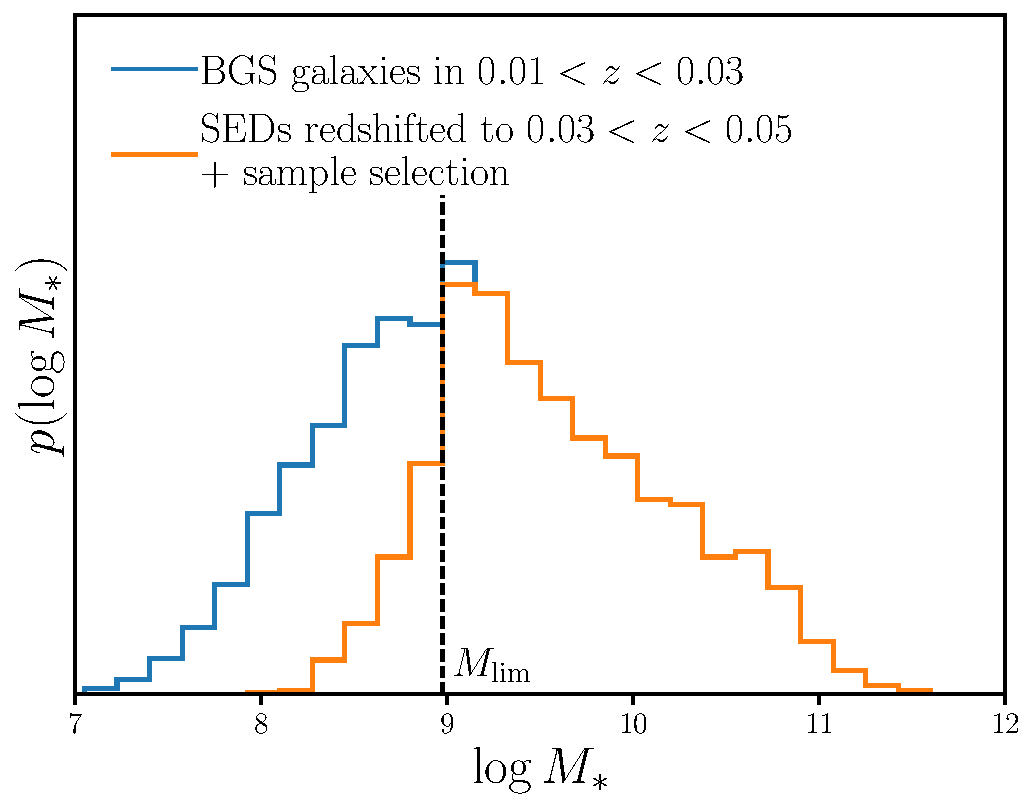
\includegraphics[width=0.45\textwidth]{figs/psmf_logMstar_comp_demo.pdf}
    \caption{blah
    }\label{fig:ms_comp0}
\end{center}
\end{figure}
%\begin{figure}
%\begin{center}
%    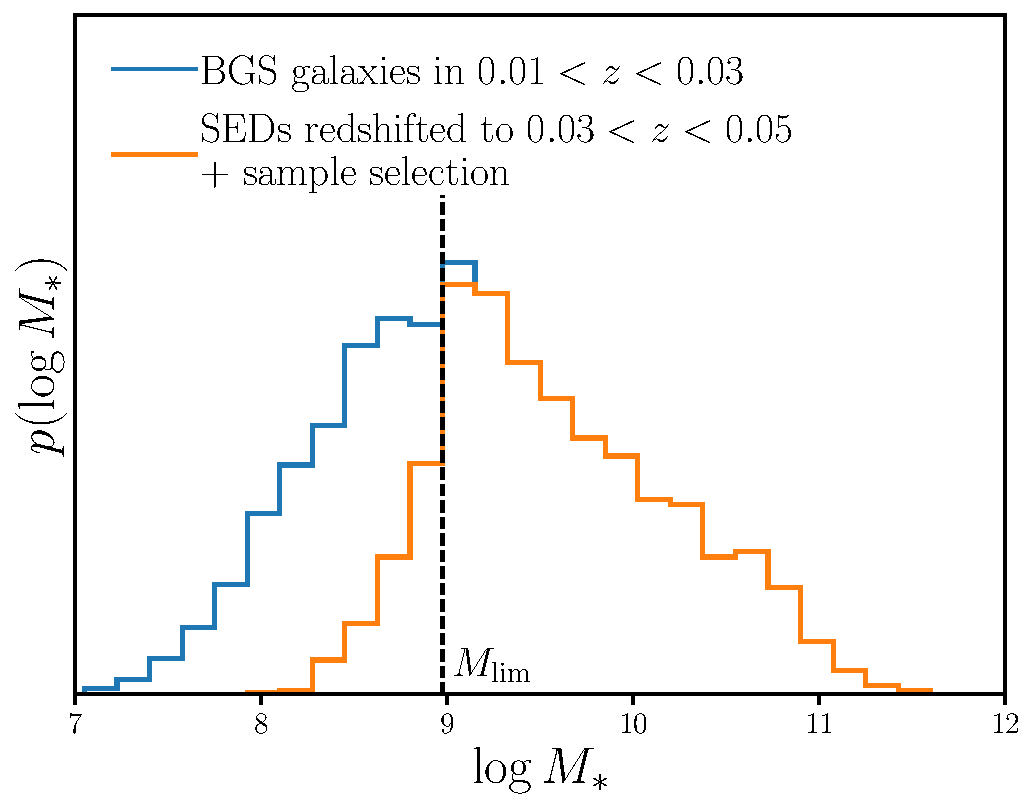
\includegraphics[width=0.5\textwidth]{figs/psmf_logMstar_comp_demo.pdf}
%    \caption{
%        To determine the $M_{\rm lim}$, the $M_*$ completeness limit, we
%        galaxies in redshift bin
%    }\label{fig:ms_comp0}
%\end{center}
%\end{figure}


%\begin{figure}
%\begin{center}
%    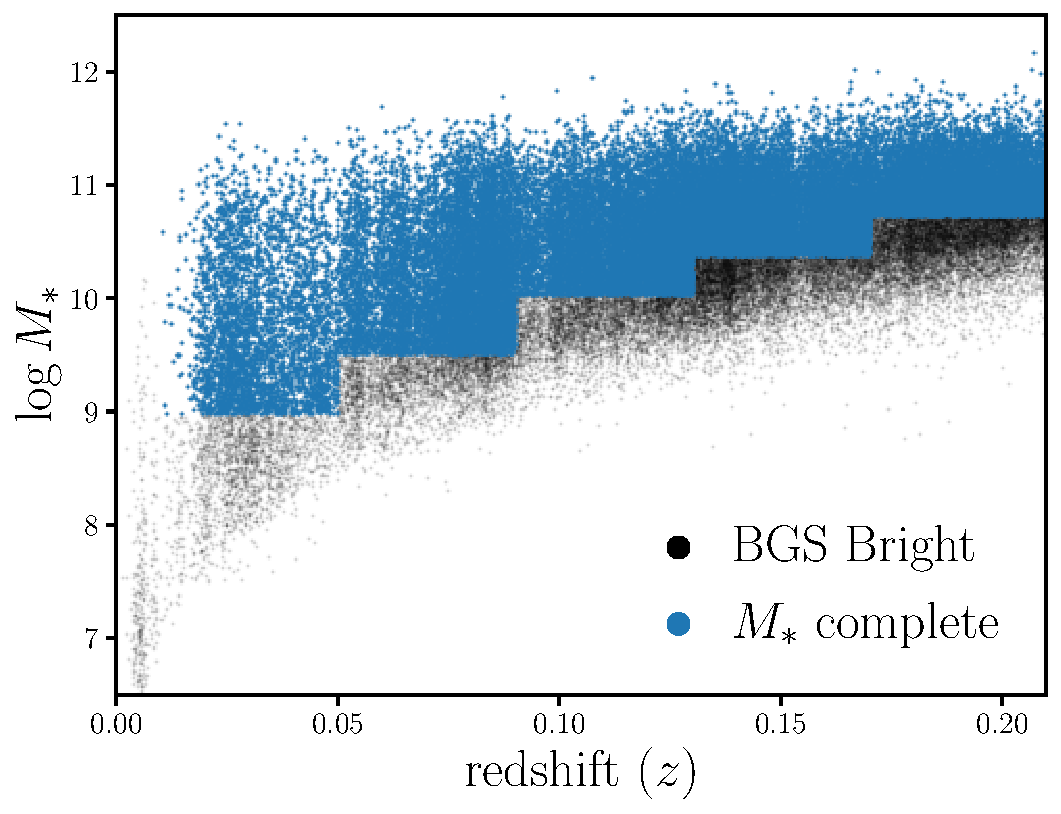
\includegraphics[width=0.6\textwidth]{figs/psmf_logMstar_comp_z.pdf}
%    \caption{
%    }\label{fig:ms_comp1}
%\end{center}
%\end{figure}


\bibliographystyle{mnras}
\bibliography{psmf} 
\end{document}
